\section{Vorwort}
Bei der Recherche zur Bearbeitung der Übungen wurden viele englischsprachige Webseiten zu rate gezogen. Generell kann man sagen, dass englische Fachbegriffe sich im Bereich FPGA und embedded Design etabliert haben, so dass eine Übersetzung eher verwirren als helfen würde. Daher haben wir uns entschieden, die \textbf{englischen} Bezeichner und Beschreibungen beizubehalten.\\
Um Codeabschnitte besser von Beschreibungen besser unterscheiden zu können, wurde eine eigene Schriftart verwendet:
\begin{verbatim}
  Kommandozeilen Eingaben und Codesnippets werden wie HIER dargestellt.
\end{verbatim}

\section{Aufgabe 1} \label{ex1}
In der Laborübung wurde ein IP Core, welcher in C Code beschrieben wurde, durch HLS eingesetzt.


\subsection {HLS Theorie}
High-Level-Synthese (HLS) verbindet Hardware- und Software-Domänen zusammen. Entwickler können so die Vorteile der Hardwareimplementierung direkt aus den Verhaltensweisen des Algorithmus ziehen, die in C-ähnlichen Sprachen mit hohem Abstraktionsgrad angegeben werden. Um die Leistungslücke zwischen den manuellen und HLS-basierten FPGA-Designs zu verringen, werden in den heutigen HLS-Werkzeugen verschiedene Code-Optimierungsformen bereitgestellt. \\


\subsection {Beschreibung}
Das Musterdesign ist ein FIR-Filter. Das muss in HLS-Software synthetisiert und als IP gespeichert werden.\\

\subsection {Die Zahl der Zyklen von dem Code}
Die Latenzverzögerung ist auf die RTL Logik zurückzuführen, die aus der mit Shift\_Accum\_Loop bezeichneten Schleife synthetisiert wird. Die Schleife wird 11 mal ausgeführt (Trip Count). Jede Ausführung erfordert 7 Taktzyklen (Iteration Latency) für insgesamt 77 Taktzyklen, um alle Iterationen dieser Schleife synthetisierten Logik (Latency) auszuführen.\\
 7 * 11 = 77 \\

\begin{minipage}{\textwidth}
    \begin{center}        
        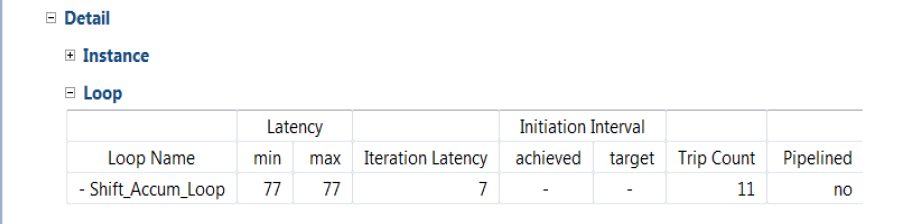
\includegraphics[scale=0.7]{img/Latency.png} 
    \end{center}
\end{minipage}
\begin{center}
Leistungsschätzung
\end{center}

\subsection {die benötigten Ressourcen}
Der Entwurf verwendet einen einzelnen Speicher, der als LUTRAM implementiert ist, 4 DSP48s und  243 Flip-Flops und LUTs.\\

\begin{minipage}{\textwidth}
    \begin{center}        
        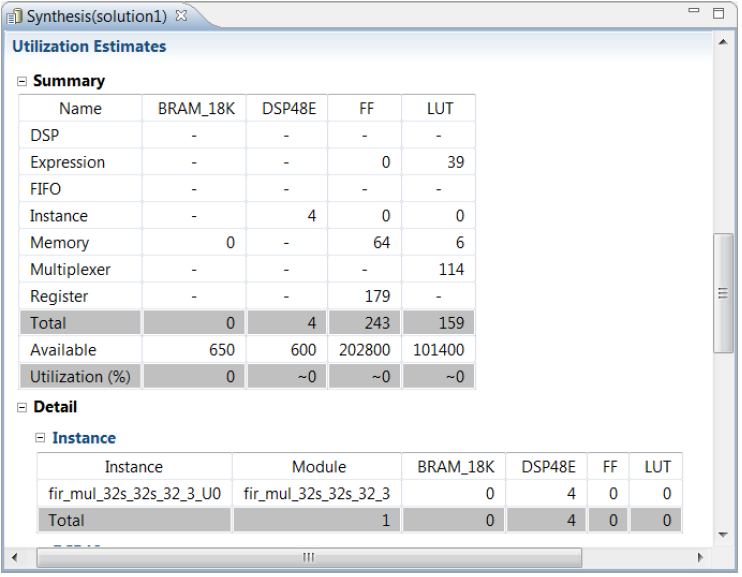
\includegraphics[scale=0.7]{img/Utilization.png} 
    \end{center}
\end{minipage}
\begin{center}
Nutzungsschätzungen
\end{center}


\subsection {Eine Multiplikation
mit vier DSP48E}
Da es sich bei den Daten um einen C-Integer-Typ handelt, der 32-Bit ist. Dies führt zu großen Multiplizierern.Ein DSP48-Multiplizierer ist 18 Bit und erfordert mehrere DSP48, um eine Multiplikation für Datenbreiten von mehr als 18 Bit zu implementieren.\\

\begin{minipage}{\textwidth}
    \begin{center}        
        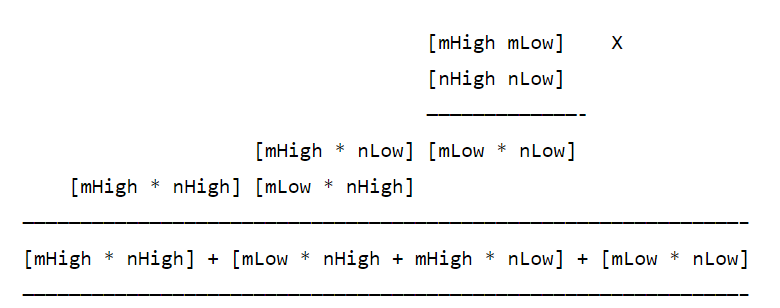
\includegraphics[scale=0.7]{img/split32bits_4dsp.png} 
    \end{center}
\end{minipage}
\begin{center}
Multiplikationsformel
\end{center}

\begin{minipage}{\textwidth}
    \begin{center}        
        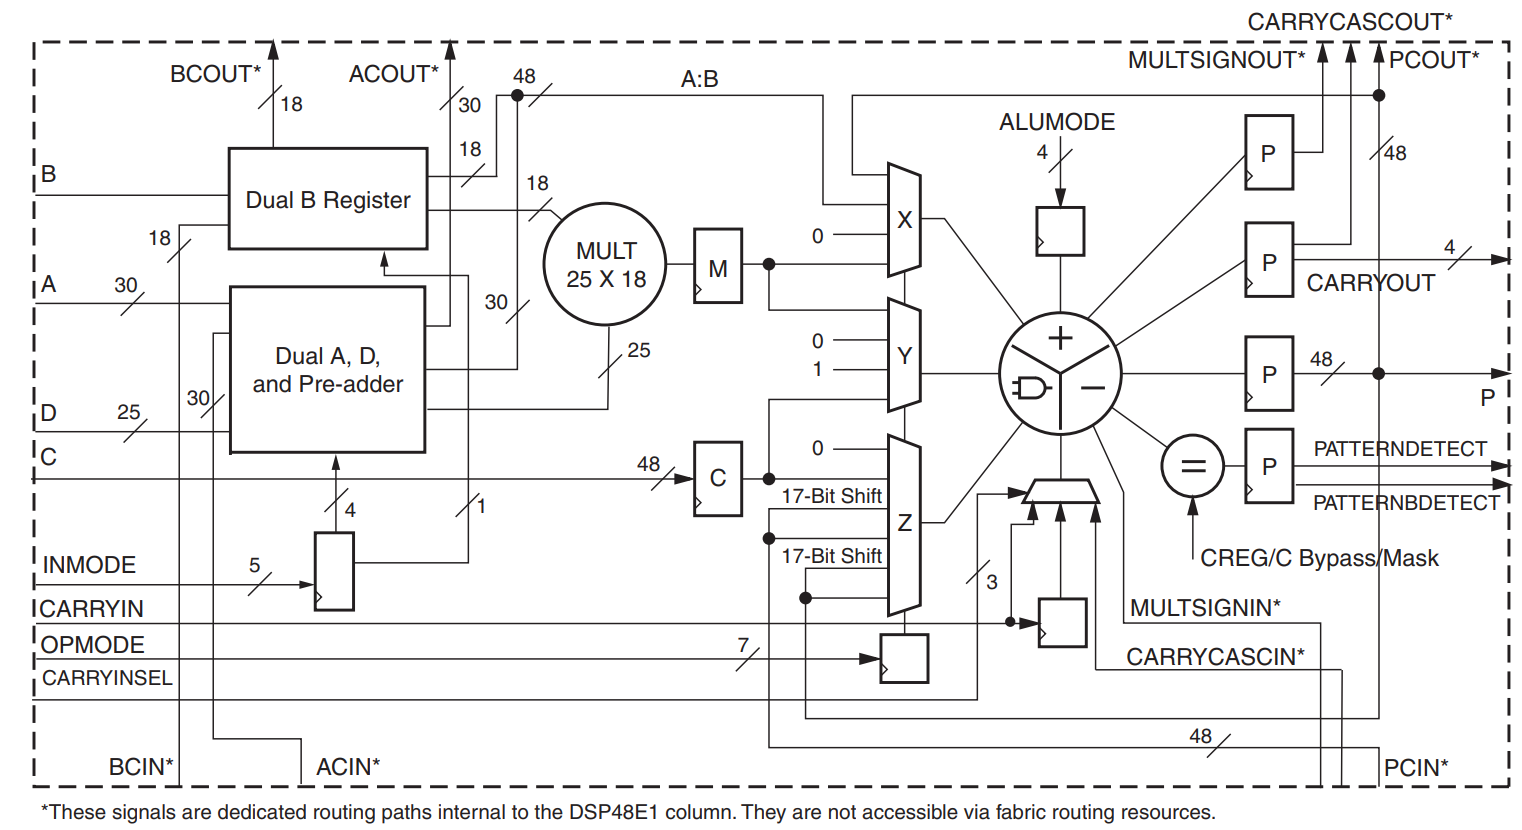
\includegraphics[scale=0.4]{img/DSP48e.png} 
    \end{center}
\end{minipage}
\begin{center}
DSP48e
\end{center}



\subsection {die benötigten Operationen des Design und deren Laufzeit}
In der linken Feld der Performance\-Ansicht werden die Operationen im Modul der RTL\-Hierarchie angezeigt.\\


\begin{minipage}{\textwidth}
    \begin{center}        
        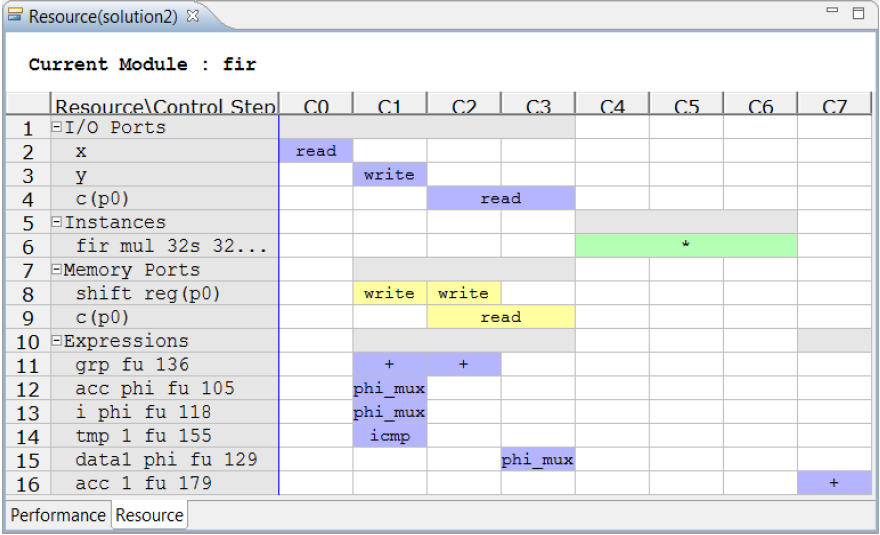
\includegraphics[scale=0.64]{img/Resource.png} 
    \end{center}
\end{minipage}
\begin{center}
Quellen
\end{center}
\begin{minipage}{\textwidth}
    \begin{center}        
        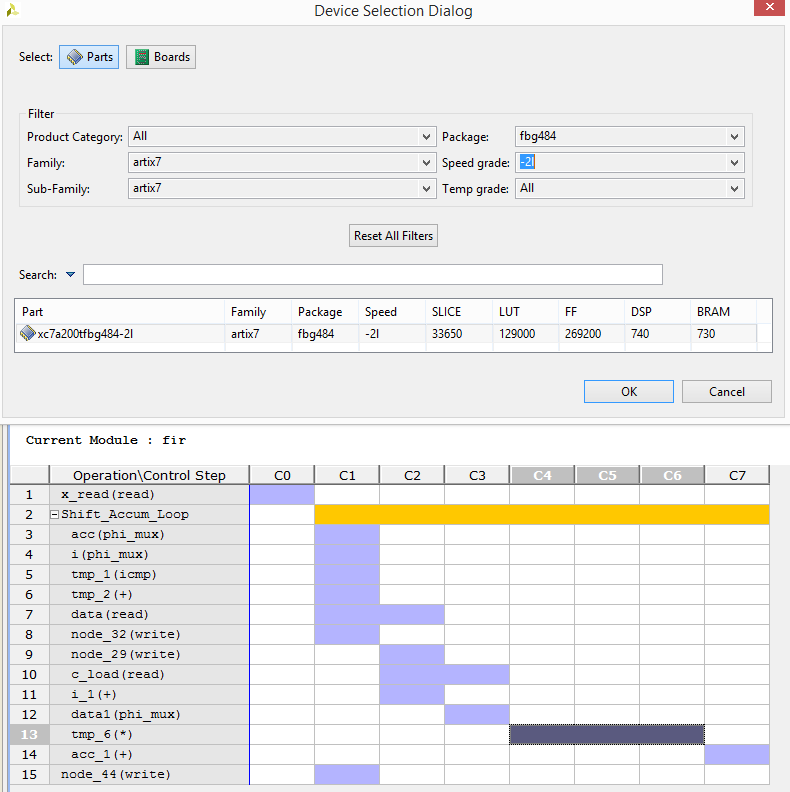
\includegraphics[scale=0.7]{img/simu.png} 
    \end{center}
\end{minipage}
\begin{center}
Performanz
\end{center}

